\subsection{Needle variations}
In the beginning of section 3 we talked about the variations of trajectories, and analyzed those variations \textit{a-posteriori}, trying to describe them. Now we are going to see, so to say, \textit{the elementary (infinitesimal) way of producing said variations.} This will be of course through control variations, not through the variation of initial condition.


\paragraph{Needle variation (fixed interval)}
et \controlSystem be a control system, $x_0\in\chi$ be an initial condition for eq. \ref{e1.1}, $\tzto\subset\R$ a time interval, $\mu\in\admContr{x_0,t_0,\tzto}$. We then define 
\lista{
	\item \grass{fixed interval needle variation \underline{data}} as a triple $\theta=(\tau_\theta,l_\theta,\omega_\theta)$ for which \lista{
		\item $\tau_\theta\in(t_0,t_1]$
		\item $l_\theta\in\R_{\geq0}$
		\item $\omega_\theta\in U$
	}

	\item the \grass{control variation} of the control $\mu$ associated to the relative fixed interval needle variation data $\theta$ is the map $\mu_\theta$ is the map $mu_\theta:J\times\tzto\fd U$ such that
	\[\mu_\theta = \left\{ \begin{array}{lr}
	\omega_\theta & \mbox{if $t\in[\tau_\theta-s*l_\theta,\tau_\theta]$}\\
	\mut & \mbox{otherwise}.\end{array}
	\right.	\]
	Where $J=[0,s_0]$ is an interval sufficiently small so that $\mu_\theta(s,t)$ is an admissible control for each $s\in J$
	Just to have an idea, this is how the function $\mu_\theta$ can look like for a certain $s>0$
	\begin{figure}[H]
		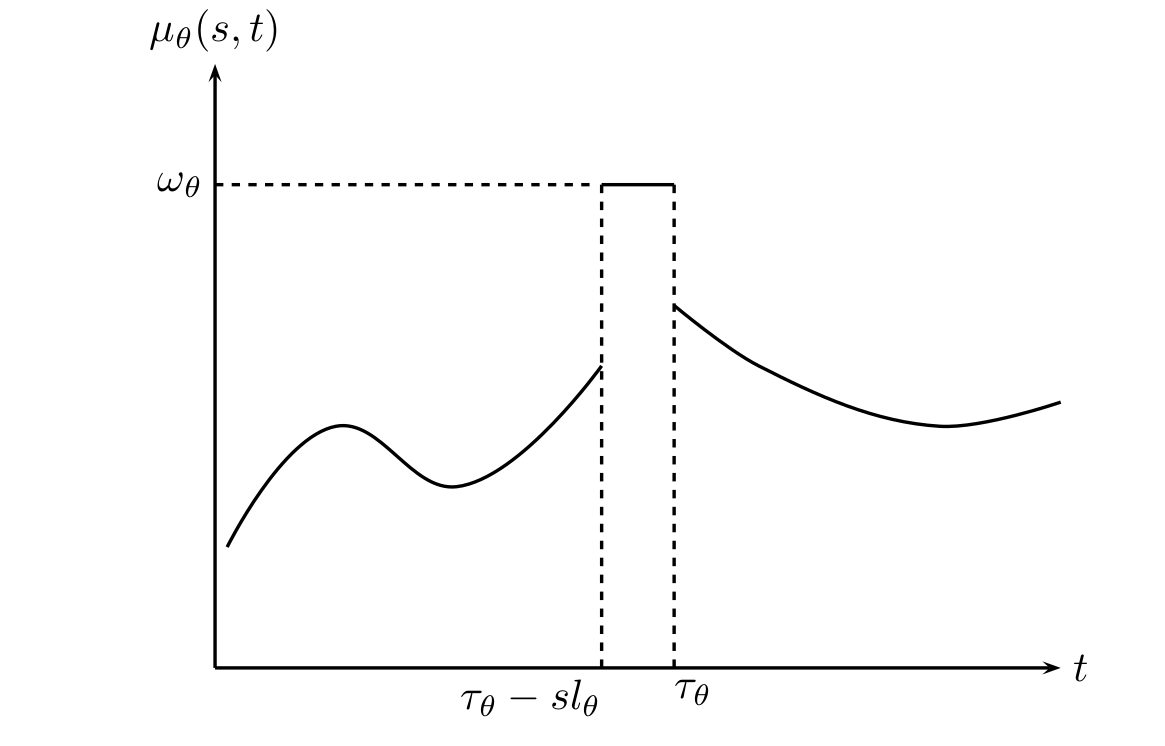
\includegraphics[width=\linewidth]{imgs/needle-variation.png}
		\caption{}
		\label{fig-needle-variation}
	\end{figure}
	\item \grass{fixed interval needle (\textit{infinitesimal})variation} associated with the control $\mu$, the trajectory \trajWinCond{\cdot} and the variation data $\theta$ as a vector of $\R^n$ defined as 
	\[v_\theta = \frac{d}{ds}\bigg|_{s=0} \xi(\mu_\theta(s,\cdot),x_0,t_0,\tau_\theta),\] when such derivative exists
}
This limit exists at almost any instant, since it exists for every instant that is a Lebesgue point for $t\fd f(\trajWinCondMath{t},\mut)$. Before stating this formally, we need the definition of $Leb(\mu,x_0,t_0,t)$: it's the set of Lebesgue points if $\tau\fd f(\trajWinCondMath{\tau},\mu(\tau)), \tau\in(t_0,t)$. Then,

\paragraph[prop 4.9]{Theorem:existence and form of fixed interval needle variations}\mbox{}\\
Let \controlSystem be a control system, $x_0\in\chi$ be an initial condition for eq. \ref{e1.1}, $\tzto\subset\R$ a time interval, $\mu\in\admContr{x_0,t_0,\tzto}$. Let then $\theta=(\tau_\theta,l_\theta,\omega_\theta)$ be a fixed interval needle variation data, with $\tau_\theta\in Leb(\mu,x_0,t_0,t_1)$. Then the fixed interval variation associated with those data exists and it's given by
\[ v_\theta=l_\theta*\bigg(f(\trajWinCondMath{\tau_\theta},\omega_\theta) - f(\trajWinCondMath{\tau_\theta},\mu(\tau_\theta) )  \bigg) \]

\subparagraph[4.10]{Variations and cones} The real importance of this theorem is not only in the fact that it is (almost) always possible to individuate the infinitesimal variation, but also in the fact that those variations form a cone, which is, if one vector represents a variation, then all of the half-line (originating from $0\in\R^n$) given by that vector is made up of fixed interval variations. Formally said, \\\\

\grass{Proposition:} Let \controlSystem be a control system, $x_0\in\chi$ be an initial condition for eq. \ref{e1.1}, $\tzto\subset\R$ a time interval, $\mu\in\admContr{x_0,t_0,\tzto}$. Let then \fivData be a fixed interval needle variation data, with $\tau_\theta\in Leb(\mu,x_0,t_0,t_1)$.\\
Then, the set of fixed interval needle variation associated with the data $\theta$ form a cone.\\\\
\grass{Proof:} It's just enough to say that, if $v_\theta$ is the variation associated with the data \fivData, then, taken a $k\in\R_{\geq0}, kv_\theta$ is the variation associated with the data $k\theta=(\tau_\theta,k*l_\theta,\omega_\theta)$. Using obvious notation, one could then say that $v_{k\theta}=kv_\theta$.\\\\
It is interesting to note that, in the triple representing the data, only the \textit{"lenght of the disturbance"} gets multiplied by the scalar. This means, that, referring to \ref{fig-needle-variation}, the final control is practically the same. In fact, the actual length of the horizontal step in the figure doesn't really matter, since s tends to zero, and the actual disturbance gets reduced to a (Lebesgue-neglettable) single point in time. \\
The only effect one may obtain is that, given a certain trajectory, the trajectories associated with varied control depart from the undisturbed one at a higher rate with growing s (at least, as long as s is small enough so that one can linearize the effect of control variation), but in the same direction. This is the same exact meaning of the length of the dotted arrows in \ref{fig-variations}.


\subsection{Multi-needle variations}
The concept behind multi needle variations is that they are made of single needle variations which sum up(linearly, as can be see in the relative theorem). We need this object basically because although single needle variations do form a cone, this is not generally convex. Convexity is needed in the proof, to find a hyperplane that separates the half space containing cone from another one. This is because a variational cone originating from the boundary of the reachable set cone will point toward the "less optimal", this half space is the non optimal one.\\\\
So now let \controlSystem be a control system, $x_0\in\chi$ be an initial condition for eq. \ref{e1.1}, $\tzto\subset\R$ a time interval, $\mu\in\admContr{x_0,t_0,\tzto}$. We want to define
 \lista{
	\item the \grass{fixed interval multi-needle variation data $\Theta$} as the collection $\Theta=\{\theta_1,..,\theta_k\}$ of fixed interval needle variation data $\theta_j=(\tau_j,l_j,\omega_j),j=1,..,k$, with the times $\tau_j$ all distinct.
	
	\item the \grass{control variation} of the control $\mu$ associated with the relative data $\Theta$ as the map $\mu_\Theta:J\times\tzto\fd U$ such that
	\[\mu_\Theta = \left\{ \begin{array}{ll}
	\omega_j & \mbox{if $t\in[\tau_\Theta-s*l_\Theta,\tau_\Theta],j=1,..,k$}\\
	\mut & \mbox{otherwise}.\end{array}
	\right.	\]
	Where $J=[0,s_0]$ is an interval sufficiently small so that $\mu_\Theta(s,t)$ is an admissible control for each $s\in J$.
	
	\item the \grass{fixed interval multi-needle variation} associated with the control $\mu$, the trajectory \trajWinCond{\cdot}, the time $t\in\tzto$ taken such that $t>\underset{j}{\max}(\tau_j)$ and the variation data $\Theta$ as a vector of $\R^n$ (a vectorial function of time actually) defined like this: 
	\[v_\theta(t) = \frac{d}{ds}\bigg|_{s=0} \xi(\mu_\Theta(s,\cdot),x_0,t_0,t),\] when such derivative exists
}

\paragraph[4.12]{Theorem: existence of multi-needle fixed interval variations}\mbox{}\\
Let \controlSystem be a control system, $x_0\in\chi$ be an initial condition for eq. \ref{e1.1}, $\tzto\subset\R$ a time interval, $\mu\in\admContr{x_0,t_0,\tzto}$. Then, let $\Theta=\{\theta_1,..,\theta_k\}$ be a multi needle variation data ("fixed interval" will from now on be omitted, since this case is the only one treated in this essay),$\Theta$ such that the times $\tau_j\in Leb(\mu,x_0,t_0,t)$, are all distinct, and also $t>\underset{j}{\max}(\tau_j)$.\\
Then, the multi needle variation is given by
\[v_\Theta(t)=\sum_{j=1}^{k}\fondMatMath{\tau_j}{t}\cdot v_{\theta_j} \]
As one can see, the variations caused by the various single needle variations first are let evolve in time from the instant in which they are applied to the "current" one, $t$, and then their effects sum up linearly.\\\\
Taking this into account, and also considering the fact that $v_{k\theta_j}=kv_{\theta_j}$ for whatever $k\geq0$ real, and remembering that the matrix-vector product is linear with respect to scalar multiplication, one can easily get the following
\subparagraph[4.13]{Corollary: coned convex combination of multi needle variations} With slight abuse of notation, given the usual control system, admissible control, initial condition, interval, given a multi needle variation data with its distinct times being Lebesgue points for $f$, and with a $t>\underset{j}{\max}(\tau_j)$, given a set $\lambda=\{\lambda_1,..,\lambda_k\}\subset\R_{\geq0}$ then
\[ v_{\lambda\Theta(t)}=\sum_{j=1}^{k}\lambda_j\fondMatMath{\tau_j}{t}\cdot v_{\theta_j} \]


\subsection{Cones and reachable set}
The proof of maximum principle will deal with the \textit{"approximation of reachable set using cones"}, which is to say that at its boundary the reachable set will be confused, at least in a neighborhood of a frontier point,  with a (variational) cone. The variations used will be both single and multi needle. We're going to see that the two are, in some sense, equal.\\ We just need two more definitions.\\The first one is going to be the 

\paragraph{Tangent cone} As usual, let \controlSystem be a control system, $x_0\in\chi$ be an initial condition for eq. \ref{e1.1}, $\tzto\subset\R$ a time interval, $\mu\in\admContr{x_0,t_0,\tzto}$. We then take $t\in\tzto$. Then we denote by \fixIntTanCone{t} the coned convex hull of the following set: 
\[ \cup \{ \fondMatMath{\tau}{t}\cdot v|\tau\in Leb(\mu,x_0,t_0,t)\text{where $v$ is a single needle variation at time }\tau. \} \]
In simple words, $K$ is built in the following way: by taking every single needle variation at every possible time preceding the current one(almost: they still have to be Lebesgue points), making the disturbance evolve from its origin to the current time trough matrix $\Phi$ and then by taking the coned convex hull of the set union of all those vectors. \\
We now define the analogue to \fixIntTanCone{t} but for multi needle variations.

\paragraph{Tangent r-simplex cone(and relative data)} As usual, let \controlSystem be a control system, $x_0\in\chi$ be an initial condition for eq. \ref{e1.1}, $\tzto\subset\R$ a time interval, $\mu\in\admContr{x_0,t_0,\tzto}$. We then take $t\in\tzto$. We then define 
\lista{
	\item the \grass{tangent r-simplex cone data} as a collection $\{\Theta_1,...,\Theta_r\}$ of multi needle variations. \\
	By using this notation:$\Theta_i=\{\theta_ij\};i=1,..,r;j=1,..,k_i$, we require that the times $\tau_ij$ are all distincts, are all Lebesgue points-
	
	\item given the multi needle variations $v_{\Theta_i}$associated with the relativa r-simplex cone data, the coned convex hull of ${v_{\Theta_i}$  is actually an r-simplex cone and defined as the \grass{tangent r-simplex cone}. 
}
Of course, when not explicitly said, the previous definitions where all relative to the fixed-interval case.

\paragraph[lemma 5.5]{Carac}